\section{Design}
\label{sec:design}
To create ClouDJ, we implemented the design described 
in subsections \ref{sec:architecture} and \ref{sec:execution} 
by integrating Google App Engine. 
Figure \ref{fig:arch} depicts the overall system.

\begin{figure*}[ht]
\centering
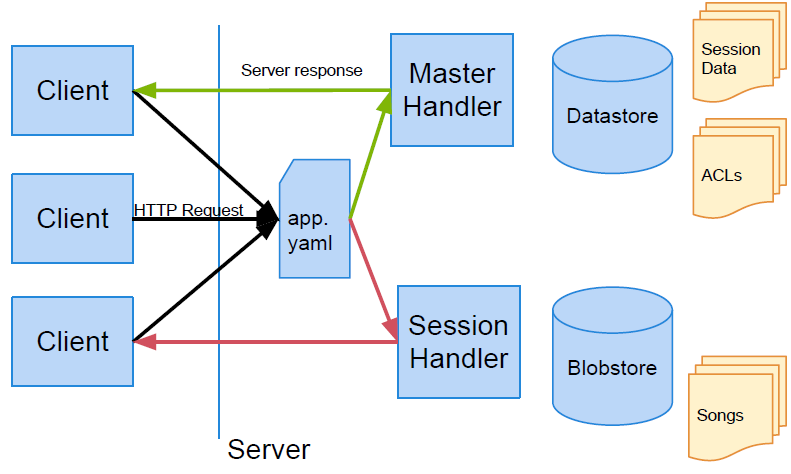
\includegraphics[width=160mm]{architecture.png}
\caption{The system architecture.}
\label{fig:arch}
\end{figure*}

\subsection{Architecture}
\label{sec:architecture}
There are three major roles in our system: 
the master handler, session handler, and client. Clients own 
and store music, can share their music with others 
and can listen to music shared by others. The master handler provides 
access control, starts sessions for users who want to host, and
connects users to their desired session. The session 
handler is in charge of handling synchronization messages between clients
and serving content.

\subsubsection{Front End}
\label{sec:frontend}
A session is an abstraction in which multiple users 
may listen simultaneously to one song that is hosted by a single user. 
Our front end (client) application allows a user to either 
create a session and become a host, or join an existing 
session and become a listener. When acting as a host, 
a user may add songs to the session playlist, 
play or pause the current song, and skip to the next song. 
When acting as a listener, the user has 
no control over what song is being played. Users can 
see all sessions that they are able to join. Only 
members of a user's access control list (ACL) may 
see or join any session in which that user is a host.

The client has access to its user's music and playlists and 
also keeps track of data such as the user's current 
session and the user's potential sessions (sessions 
this user can access). For the current session, the 
client keeps track of the session key and relevant song information. 
For the potential sessions, the client keeps the host, 
session key, and currently playing song.

\subsubsection{Back End}
\label{sec:backend}
The backend infrastructure is more complicated than 
the frontend. The master server keeps track of users 
currently online, user ACLs, and user membership lists 
(ACLs it is a member of). It also is responsible for 
adding entries to the session table, a table that keeps track
of session information including host, listeners, and current song. 
It also maintains the potential listener
list for each session. A potential listener is a client 
who could listen to the session, but is currently not. 
In other words, these are the clients on the host client's 
ACL that are logged in but not listening to this 
session. When a client logs on, the master server retrieves each 
session associated to a host on the client's 
membership list and sends back a list of sessions it could
potentially join. It also adds the client to the potential
listener list for each of those sessions.

The session handler is the workhorse of the system. It 
services requests for all sessions by routing data from the 
host client to relevant clients (listeners). It is in charge 
of maintaining the data in the session table and propagating 
commands from the host to all listeners. It is responsible
for handling uploads and serving song data. The session handler 
also takes care of session cleanup when a session ends (or 
host disconnects). 

\subsubsection{Storage}
\label{sec:storage}
Certain information is stored on the server in the Datastore and Blobstore.
Datastore holds session data and ACLs. 
Session data includes session meta data (session key, host, listeners), 
and session state (current song, song play or pause flag, session ended flag, 
timestamp of last play/next message). This information is used to coordinate
sessions among different clients. The ACLs keeps track of the potential
sessions and potential listeners for each user. Potential listeners are 
users who can listen to a session hosted by a given user and potential sessions
are sessions the user can join. Blobstore is only used 
to store song data in our application. When a session ends, the songs are deleted 
from the blobstore.

\subsection{Execution Flow}
\label{sec:execution}
As shown in Figure~\ref{fig:arch}, the general execution of the ClouDJ application
is as as follows:
\begin{enumerate}
  \item The client contacts the server
  \item The server executes the handler based on the request
  \item The handler runs and propagates updates to session participants
  \item The client receives the server response and performs actions 
\end{enumerate}

In sections \ref{sec:joinSession} and \ref{sec:playSession}, we discuss
session creation, joining and leaving sessions, and updating sessions.


\subsubsection{Creating, Joining, and Leaving a Session}
\label{sec:joinSession}
Sessions are created when a client contacts the master 
handler about hosting a new session. The master handler 
then creates a new session in the datastore and responds to the client, 
which updates its current session information. 
Clients may join sessions by contacting the master 
handler with the session key of the session they wish to join. 
The master handler updates the session information in the datastore
and notifies everyone in the session of the new listener. 
After a session is established, the client no longer communicates 
with the master handler. When a user leaves a session, the client
contacts the session handler telling it to remove itself from from
the listener list if it is not the host. If it is the host, the
session handler notifies all listeners that the session has ended and 
removes the session and corresponding song data from the datastore
and blobstore.

\subsubsection{Updating Sessions}
\label{sec:playSession}
Hosts may update the sessions using several types of messages: ``upload,''
``play,'' ``pause,'' and ``next.'' Songs are added to the session when 
the host client contacts the session handler with an ``upload'' message, 
indicating that it wants to add a song to the playlist. The session 
handler forwards the song to the blobstore and retrieves the corresponding 
blob key, which is used when requesting the song for playback. The session
handler then updates the session playlist in the datastore and sends the 
blob key to all clients in the session. The clients then fetch the song 
from the blobstore. 

Unsurprisingly, the ``play,'' ``pause,'' and ``next'' messages 
indicate when the host wants to unpause, pause, and skip the current song, respectively.
The host sends these control messages to the session handler, which updates
the session in the datastore and then propagates the message to all session
participants. The clients then peform the appropriate action. We elaborate on
playback synchronization among clients in Section~\ref{sec:sync}.

\subsubsection{Session Synchronization}
\label{sec:sync}

\begin{figure}[t!]
	\centering
	\begin{subfigure}[b]{0.5\textwidth}
		\centering
		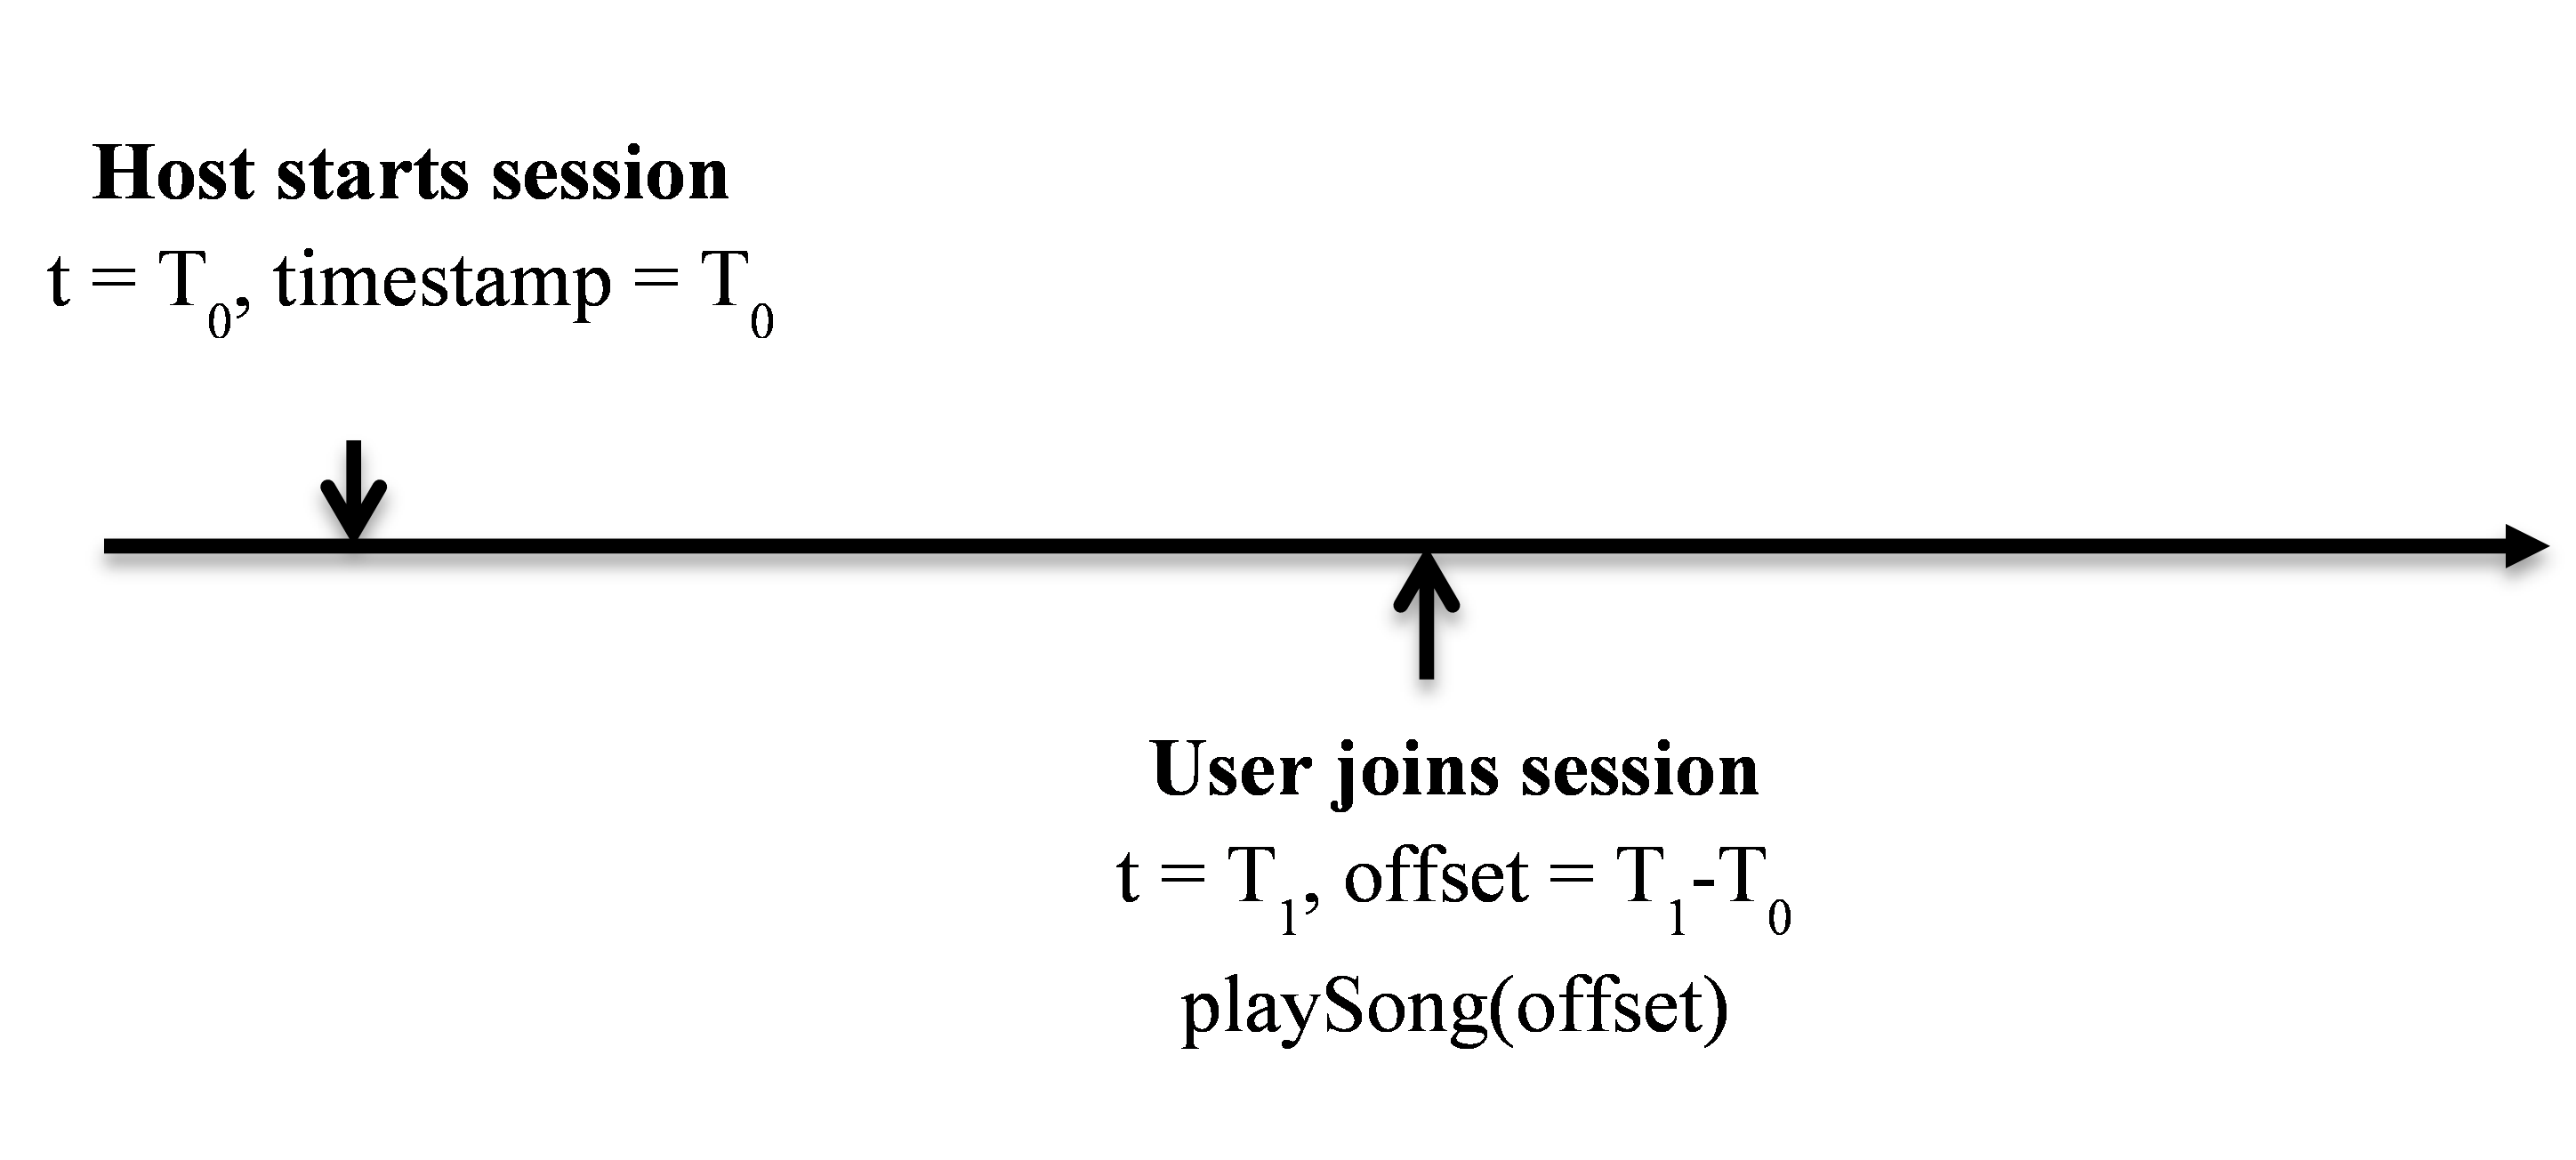
\includegraphics[width=85mm]{joinSessionPlay.png}
		\caption{Joining a session while a song is playing}
		\label{fig:syncJoinPlay}
	\end{subfigure}
	
	\begin{subfigure}[b]{0.5\textwidth}
		\centering
		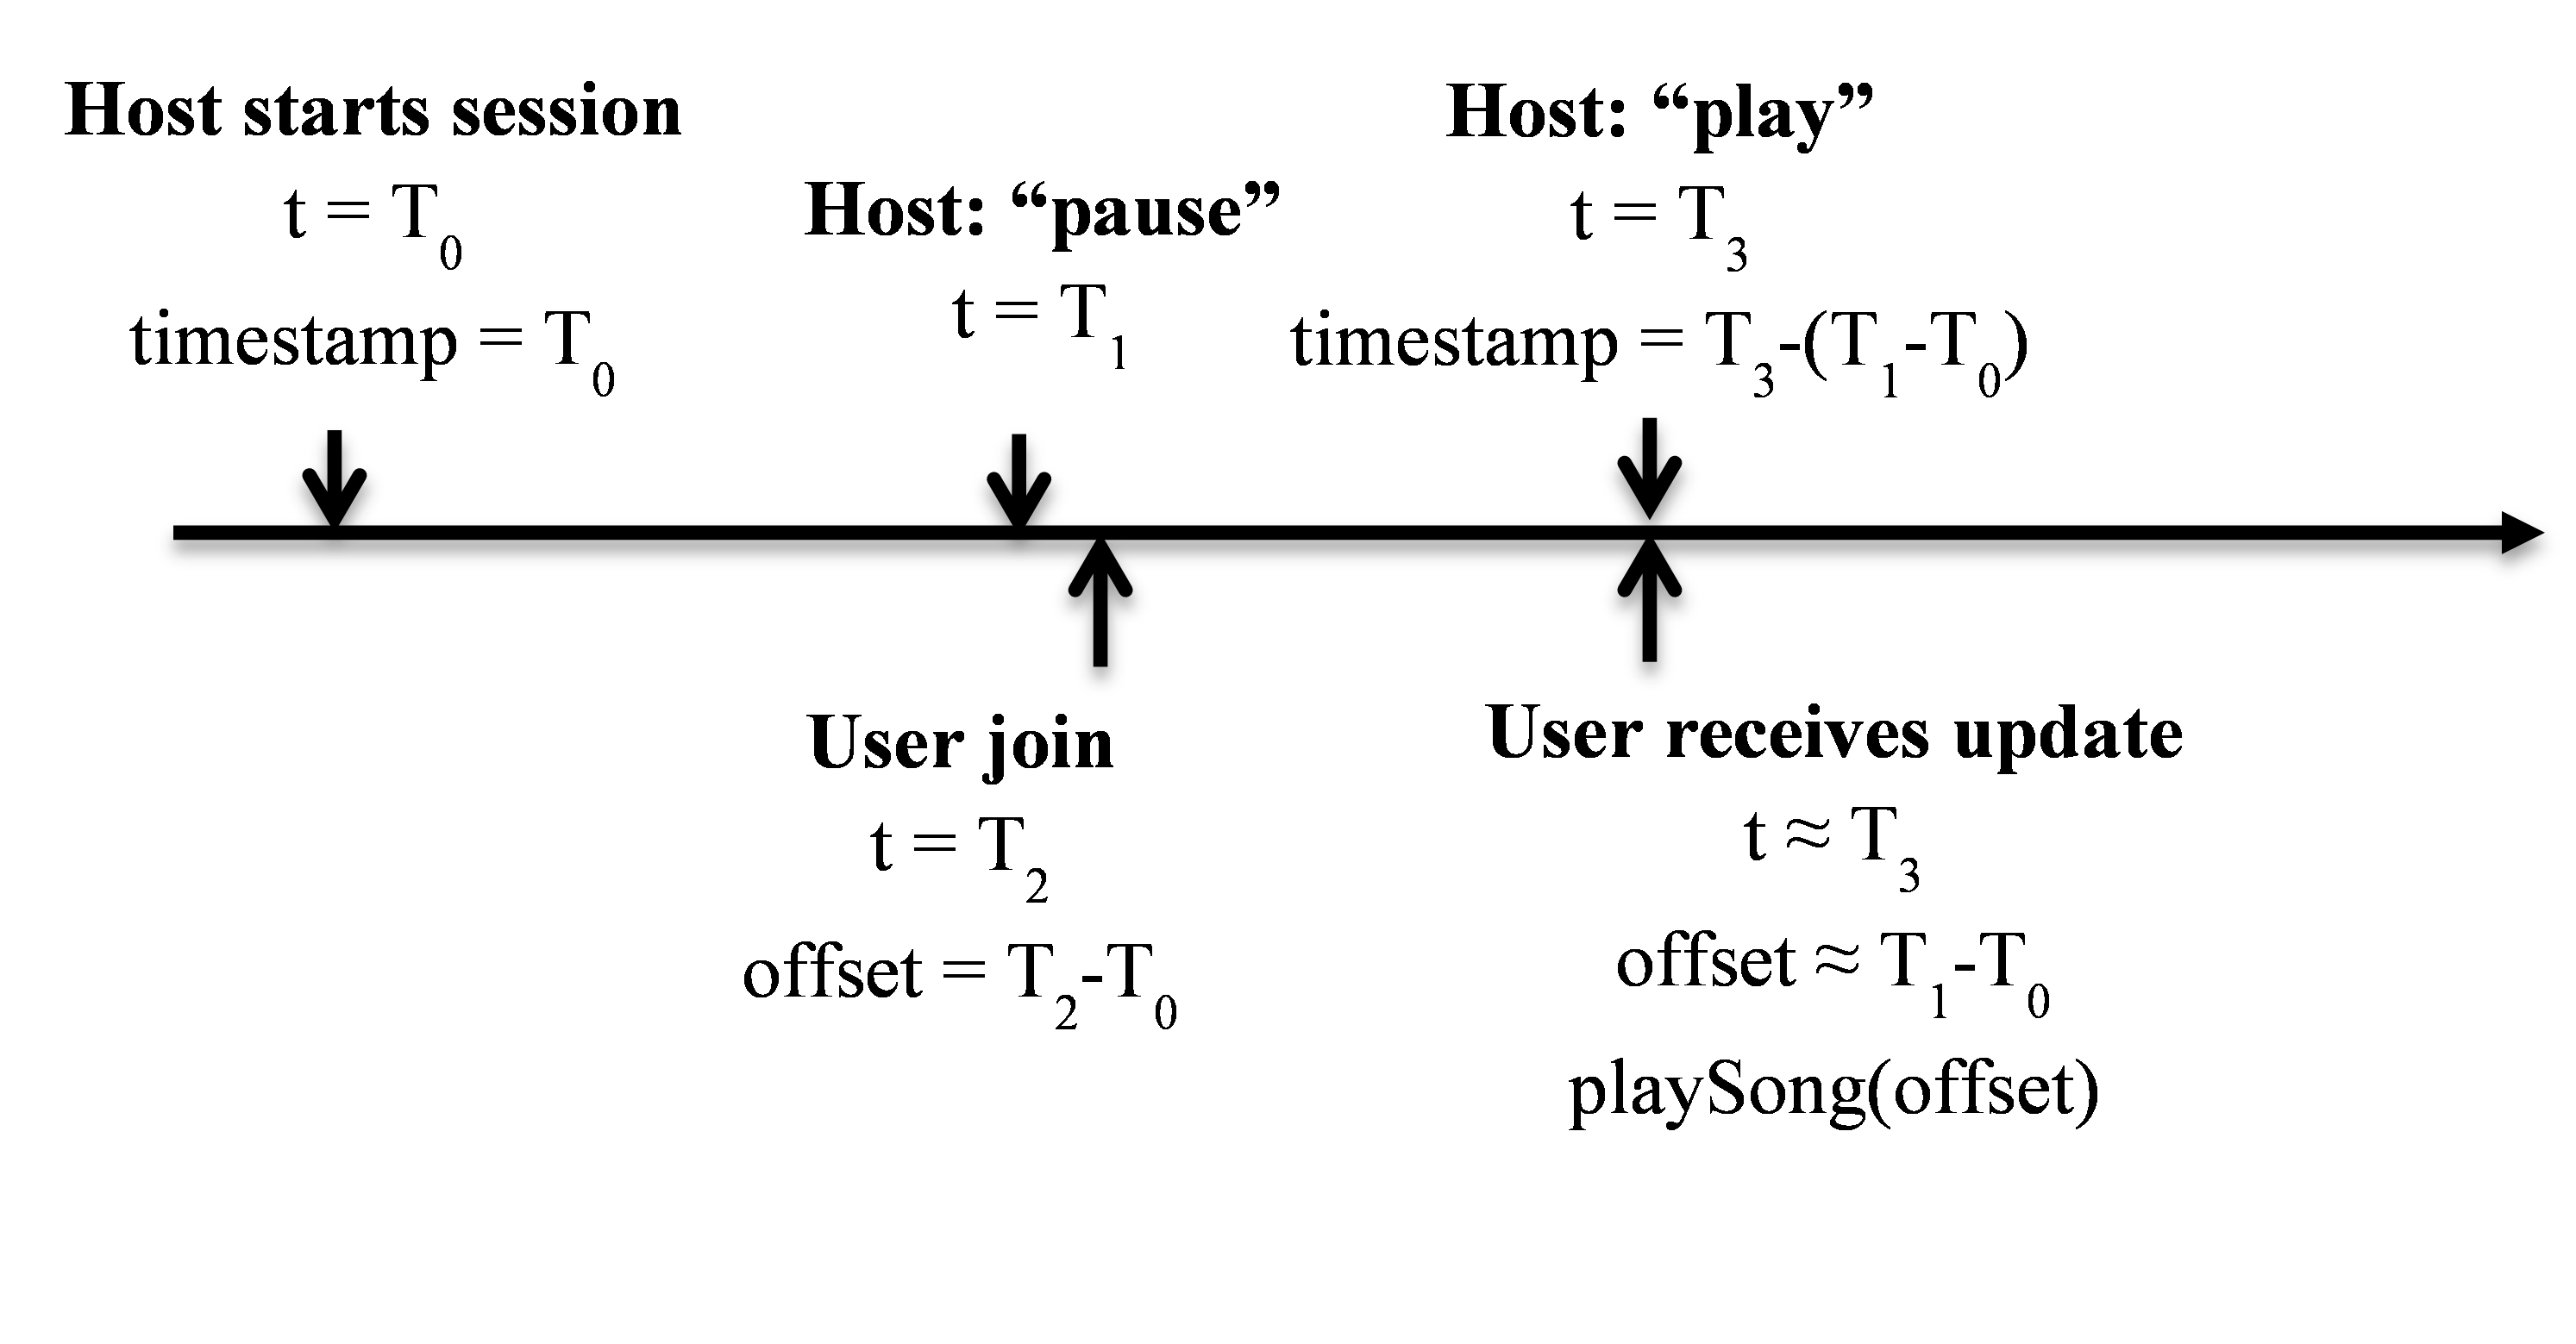
\includegraphics[width=85mm]{joinSessionPause.png}
		\caption{Joining a session while a song is paused}
		\label{fig:syncJoinPause}
	\end{subfigure}
	\caption{Synchronization messages when a user joins a session}
	\label{fig:syncJoin}
\end{figure}

In order to synchronize playback among different clients, we use 
control messages, which are propagated as described in Section~\ref{sec:channel}. 
Only hosts may issue commands such as play, pause, and 
next for the session. The ``play'' and ``pause'' commands are sent
only when the host clicks on the pause and play buttons, and the 
``next'' command is sent when the host switches songs or if the
host clicks on the ``next'' button. We separate the problem of synchronization 
into two parts: joining an existing session and updating the
current session. In both cases we utilize a timestamp, which is 
updated each time a play or next command is sent by the host client
and is sent with the control message. 

As seen in Figure~\ref{fig:syncJoin} when a user joins a session, 
the server sends the user the elapsed time since the last stored timestamp. 
The user then start the song with the value returned by the server as 
the offset. If the song is playing when the user joins the session, 
it will start playing at the specified offset. If the song is paused when 
the user joins the session, the retrieved offset will not be the correct 
elapsed time; however, this is corrected when the host sends a ``play'' 
message to the server, which stores another timestamp and propagates
the correct offset to all session listeners.

This timestamping synchronization is used mainly when a user joins a session.
In the other case where participants update their current session upon 
recieving a control message, the offset can usually be inferred based on the 
local state. For instance, if the user receives a ``next'' message, then they
start the next song with an offset of 0. If a user receives a ``pause" 
message, they stop the current song and keep the elapsed time as the offset.
If the user receives a ``play'' message they start the current song at the 
local offset, which was set when the ``pause'' message was received. The 
exception to this is if the current paused song is at the beginning, indicating
that this user has joined the session while the song was paused or that this 
user is ahead of the host and is waiting for a control message from the host. 
In this case the user adjusts the current song offset with what 
they recieve from the server. Conversely, if the listener lags behind the host, 
then they will receive a ``next'' message before the end of the song and start 
the next song. Figure~\ref{fig:syncUsers} illustrates the timeline in the cases 
where a listener is behind the host and where a listener is ahead of the host.

\begin{figure}[t!]
	\centering
	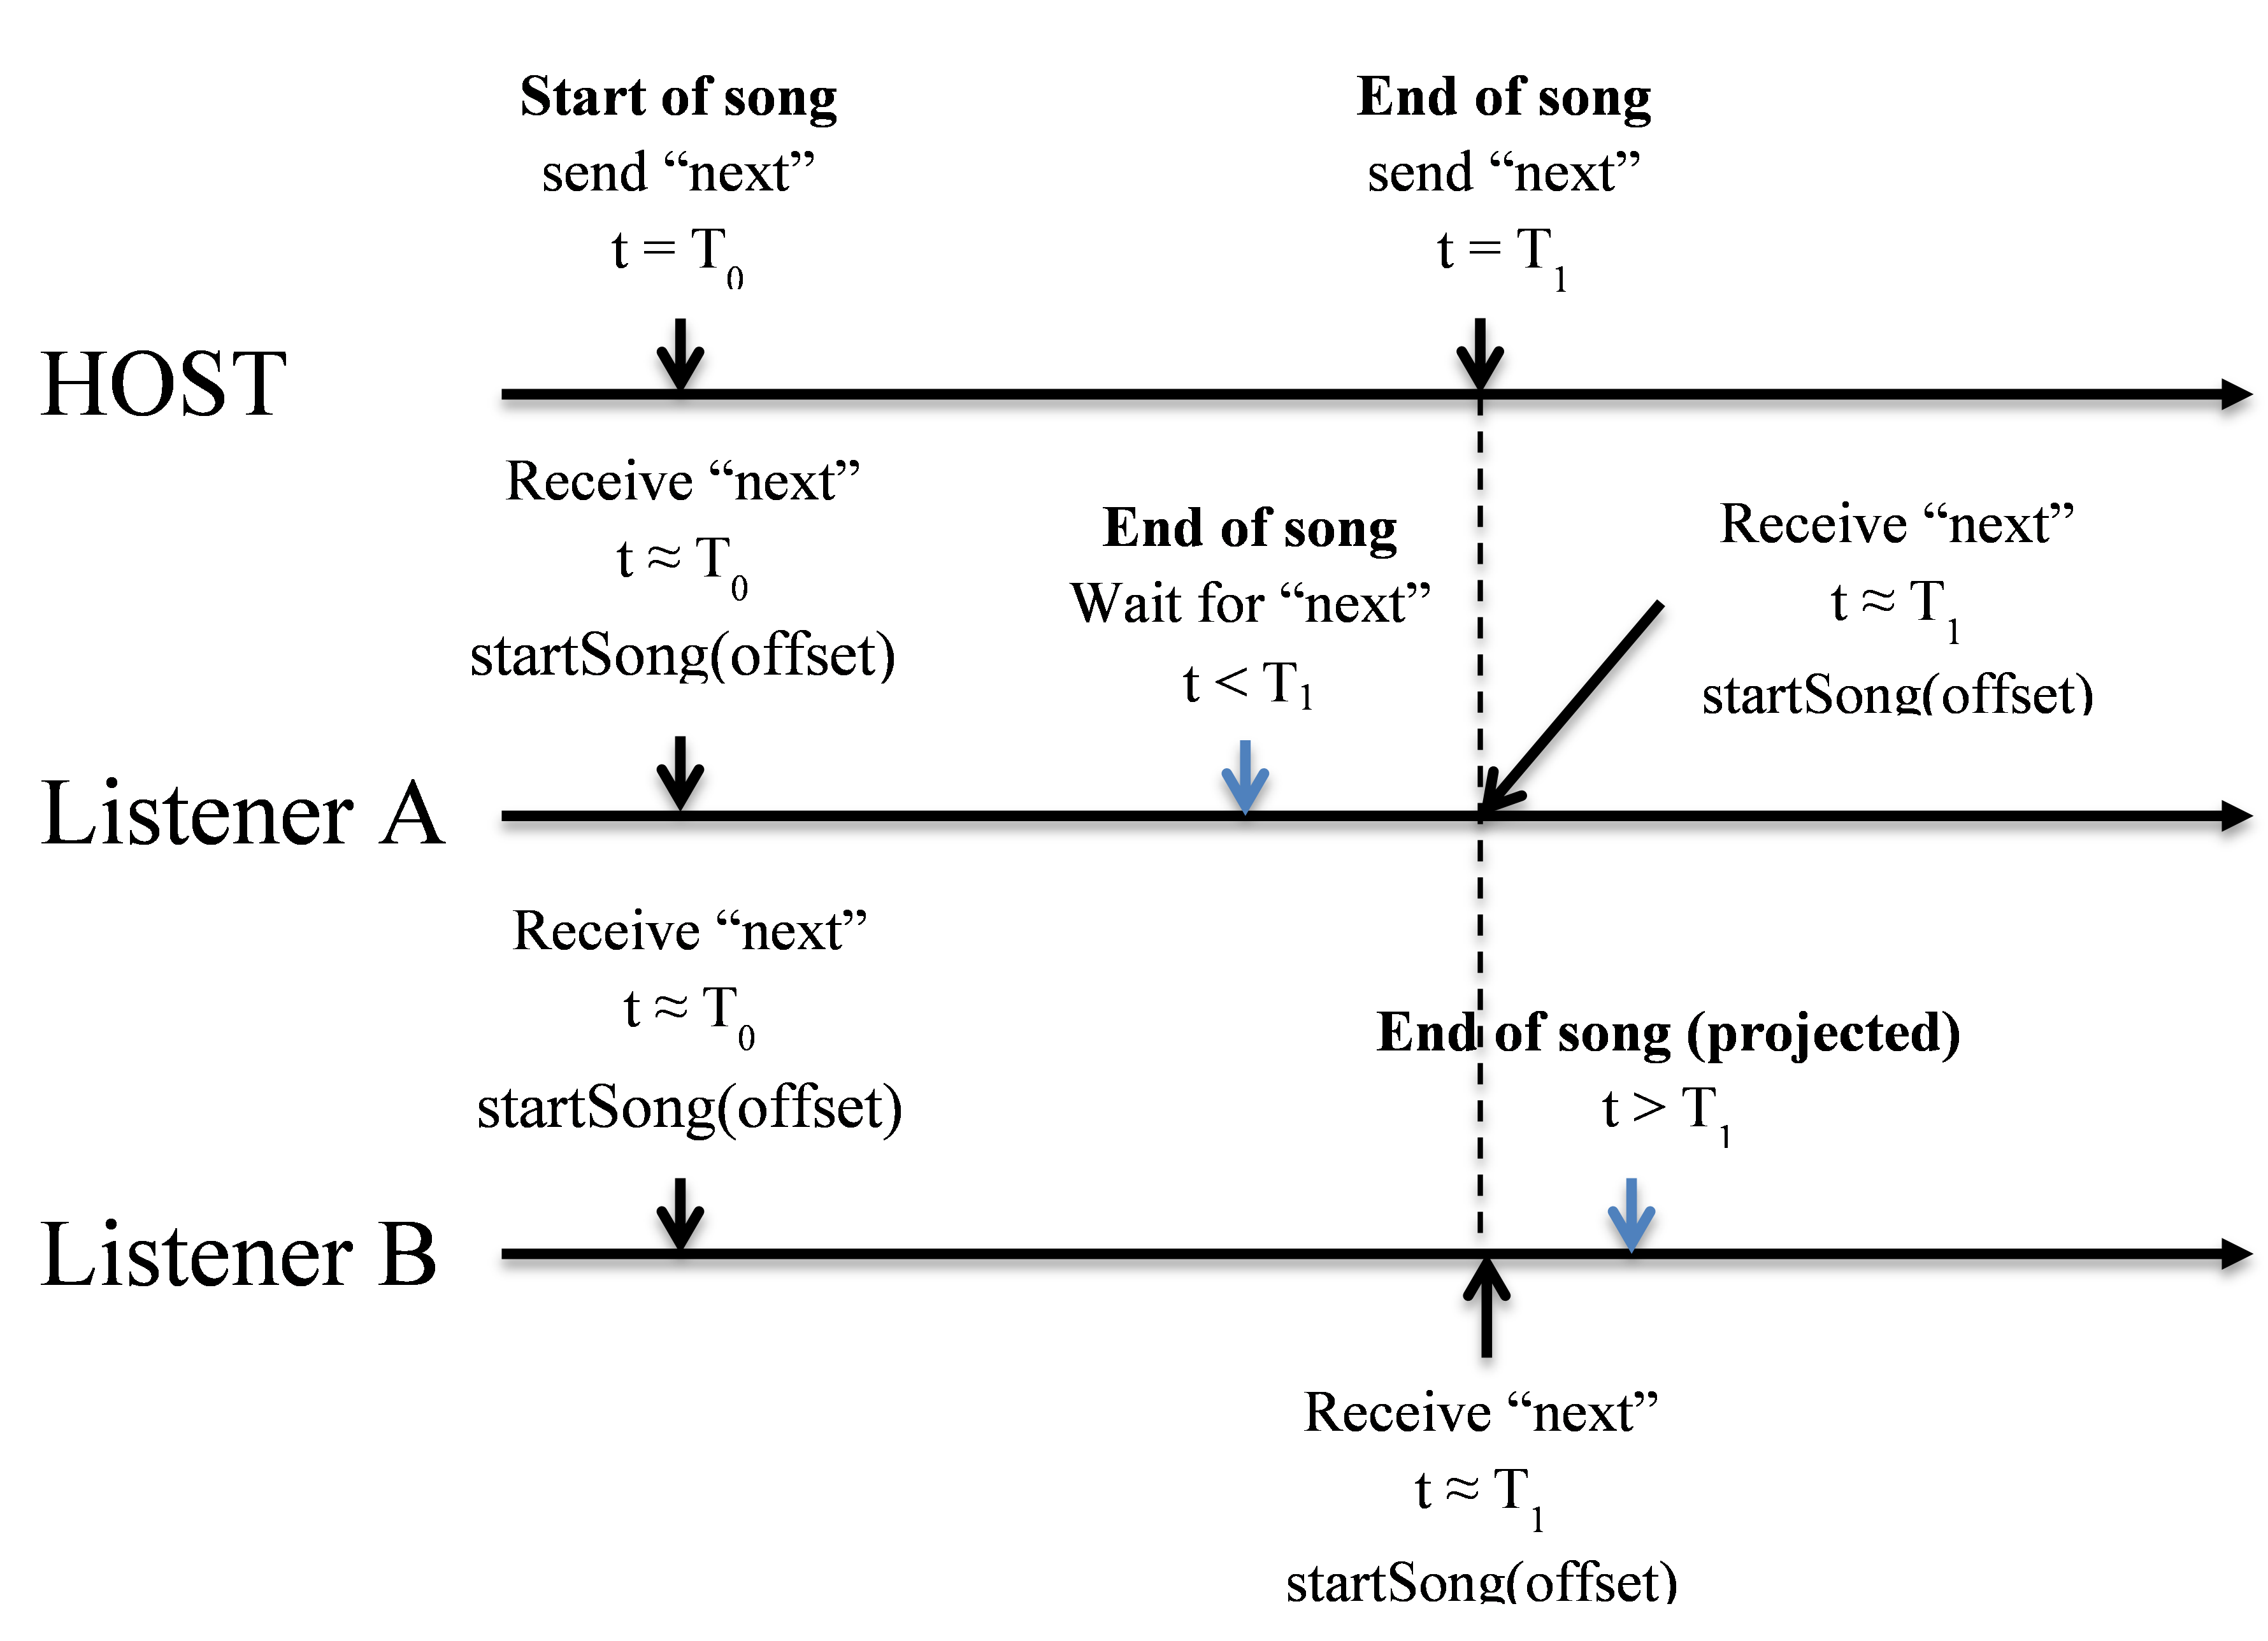
\includegraphics[width=85mm]{syncSessionUsers.png}
	\caption{The synchronization timeline for a listener that's ahead of or behind the host}
	\label{fig:syncUsers}
\end{figure}
